\documentclass[10pt,
aspectratio=169,
legacy=true,
%osgdefaults,
lang=de,
standalone,
tuc={fakcolor=if}
]{osgbeamer}

\usepackage{tikz}
\usetikzlibrary{shadows, positioning, automata, arrows, fit, arrows.meta, decorations.markings, decorations.pathreplacing, shapes.geometric, shapes.arrows,shapes.symbols}
\usepackage{amsmath}
\usepackage{exscale}
\usepackage{textcomp}
\usepackage{metalogo}
\usepackage{tabularx}

\usepackage{url}
% Trennstellen für URLs
\def\UrlBreaks{\do\:\do\.\do\@\do\\\do\/\do\!\do\_\do\|\do\;\do\>\do\]%
 \do\)\do\,\do\?\do\'\do+\do\=\do\#}
\def\UrlBigBreaks{}  


% \usepackage{listings}
% \usepackage{listingsutf8}
% \usepackage{inconsolata}
% \definecolor{javared}{rgb}{0.6,0,0} % for strings
% \definecolor{javagreen}{rgb}{0.25,0.5,0.35} % comments
% \definecolor{javapurple}{rgb}{0.5,0,0.35} % keywords
% \definecolor{javadocblue}{rgb}{0.25,0.35,0.75} % javadoc

% \lstset{
%   basicstyle=\color{blue!50!black}\ttfamily,
%   keywordstyle=\color{javapurple}\bfseries,
%   stringstyle=\color{javared},
%   commentstyle=\color{javagreen},
%   language=c,
% }

% TUC-Templates laden.
%\usetheme[fakcolor=if]{tuc2019}
%\mode<article>{\usepackage{beamerarticletuc2019}}

% Metadaten
\title{Revisiting the Laprie Model Regarding Security\\from an Industrial Perspective}
\subtitle{Frühjahrstreffen der FGBS und FERS}
\date[06.03.2023]{06.03.2023}
\institute[TU Chemnitz, OSG]{TU Chemnitz, Professur Betriebssysteme}
% \titlegraphic{\includegraphics[height=0.2\textheight]{/Users/billy/Documents/Vorlagen/logo-2014}}
\tucurl{http://osg.informatik.tu-chemnitz.de/}
\author[Christine Jakobs]{Christine Jakobs}
% linksbündig ist was feines :)
\setbeamertemplate{title page}[default][left]


\begin{document}
\tucthreeheadlines

\tucnarrowframe
\begingroup
%\logo{\includegraphics[width=\hsize]{logo-2014}}
\frame{\titlepage}
\endgroup
\tucwideframe
\tuctwoheadlines

\section{Das Problem konsistenter Terminologie}

\begin{frame}[c]
\frametitle{\emph{Fault, Error} und \emph{Failure} in der Literatur}
  \begin{center}
    %\includegraphics[width=0.6\linewidth]{definitions2}
    \begin{description}[style=sameline]\fontsize{6pt}{2pt}\selectfont
      \item[\textbf{Bildquelle:}] \stress{Tröger, Peter. Unsicherheit und Uneindeutigkeit in Verlässlichkeitsmodellen. 1. Aufl. Wiesbaden: Springer Vieweg, 2018.}
    \end{description}
  \end{center}
\end{frame} 

\begin{frame}
\frametitle{\emph{Fault, Error} und \emph{Failure} nach Laprie}
  \begin{columns}
    \column{0.5\textwidth}
    \begin{description}
      \item[Fault:] Die verantwortliche oder hypothetische Ursache für einen \emph{Error}. 
      \item[Error:]<2-> Der interne Systemzustand weicht vom korrekten Zustand ab.
      \item[Failure:]<3-> Die erbrachte Leistung des Systems weicht durch ein Ausfall-Ereignis von der beabsichtigten Leistung ab.
    \end{description}
    \column{0.5\textwidth}
    \resizebox{0.55\linewidth}{!}{
      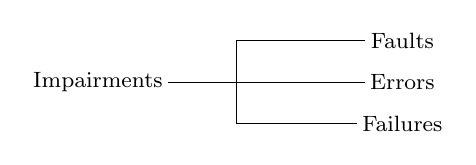
\begin{tikzpicture}[rec/.style={inner sep=2pt, outer sep=0, node
            distance=15pt, font = \footnotesize}, 
          hrec/.style={inner sep=0pt, outer sep=0, node distance=15pt}]
          
          \node[rec] at (0,0) (fault) {Faults};
          \node[rec, below of = fault](error) {Errors};
          \node[rec, below of = error](fail) {Failures};
          
          \node[rec, left of = error, node distance = 110pt](thr) {Impairments};
          
          \node[hrec, right of = thr, node distance=50pt](hthr){};
          \node[hrec, right of = thr, node distance=55pt](hthr2){};
          \draw[-](thr) -- (error.west);
          \draw[-](fault.west) -| ([yshift=-10pt]hthr.center) |- (fail.west);
          
      \end{tikzpicture}
    }
  \end{columns}
\end{frame}

\begin{frame}
\frametitle{Lapries Definition eines \emph{Faults}}
  \begin{columns}
    \column{0.5\textwidth}
\begin{itemize}
  \item Jeder \emph{Fault} liegt im Design der System Spezifikation
  \begin{itemize}
    \item[\follows] Korrekt, aber aus pragmatischem Standpunkt nicht hilfreich
  \end{itemize}
  \item <2->Unterscheidung in interne und externe \emph{Faults}
  \begin{itemize}
    \item Interne \emph{Faults} befinden sich innerhalb des Systems
    \item Externe \emph{Faults} werden von der Umgebung eingebracht
  \end{itemize}
  \item <3->Security? 
  \begin{itemize}
    \item [\follows] Interne oder externe \emph{Faults}? 
    \item [\follows] Was ist ein Angriff, eine Schwachstelle, etc.?
  \end{itemize}
\end{itemize}
    \column{0.5\textwidth}
    \resizebox{0.55\linewidth}{!}{
      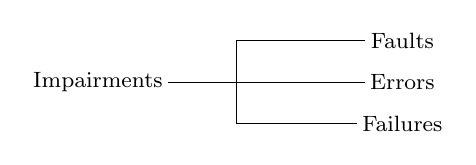
\begin{tikzpicture}[rec/.style={inner sep=2pt, outer sep=0, node distance=15pt, font = \footnotesize}, hrec/.style={inner sep=0pt, outer sep=0, node distance=15pt}]
          
          \node[rec] at (0,0) (fault) {Faults};
          \node[rec, below of = fault](error) {Errors};
          \node[rec, below of = error](fail) {Failures};
          
          \node[rec, left of = error, node distance = 110pt](thr) {Impairments};
          
          \node[hrec, right of = thr, node distance=50pt](hthr){};
          \node[hrec, right of = thr, node distance=55pt](hthr2){};
          \draw[-](thr) -- (error.west);
          \draw[-](fault.west) -| ([yshift=-10pt]hthr.center) |- (fail.west);
          
      \end{tikzpicture}
    }
  \end{columns}
\end{frame}




% \section{Security Taxonomie}

% % \begin{frame}[c]
% % \frametitle{Übertragung von Security auf das Laprie Modell}
% %   \centering
% %   \include{sectax}
% % \end{frame}


% % \begin{frame}
% % \frametitle{Security Threats}
% %   \begin{columns}
% %     \column{0.5\textwidth}
% % \begin{description}
  
% %   \item [Weakness] Interner \emph{Fault} der in die Lebenszeit des Systems propagiert und es in einen verwundbaren Zustand versetzt.
% %   \item [Attack] Böswilliger Einfluss der Umgebung welche einen externen \emph{Fault} in das System einbringt.
% %   \begin{description}
% %     \item [Attack Path] Menge von Aktionen welche beschreiben wie ein Angreifer dem System Schaden zufügt.
% %   \end{description}
% %   \item [Vulnerability] Inkorrekter Zustand in welchem das System angreifbar für böswillige externe \emph{Faults} ist. 
% %   \item [Damage] A successful attack can lead to a system state where the system behavior regarding one or more security objectives deviates from the intended one, recognizable by the user.
% % \end{description}
% % \end{frame}

% \begin{frame}[t]
% \frametitle{Security Threat Chain}
%   \centering
%   \resizebox{0.7\linewidth}{!}{
%     \begin{tikzpicture}[aut/.style={state, circle, align=center, inner sep = 1mm, font=\footnotesize}, hrec/.style={inner sep=0pt, outer sep=0, node distance=15pt}]
        
%         \node[hrec](design) at (0,0){};
%         \node[aut, right of=design, node distance=4cm](vul){Vulner-\\ability}; 
%         \node[aut, right of=vul, node distance=4cm](att){Ongoing\\ Attack};
%         \node[aut, below of=att, node distance=3cm](detect){Detected\\ Attack};
%         \node[aut, accepting, right of=att, node distance=4cm](dam){Damage};
        
%         \draw(vul) edge[loop above] (vul);
%         \draw(att) edge [-latex] node[midway, font=\footnotesize,xshift=-0.8cm]{\textit{Detection}} (detect);
%         \draw(design) edge [-latex] node[midway,above,xshift=-0.5cm, align=center, text width=1.3cm, font=\footnotesize, name=weak]{\textit{Internal/External\\ Weakness}} (vul);
%         \draw(detect) edge [-latex] node[midway,  text width=1.5cm, align=center, xshift=-1.1cm,  yshift=-0.3cm, font=\footnotesize ]{\textit{Successful\\ Attack\\ Handling}} (vul);
%         \draw(detect) edge [-latex] node[midway, font=\footnotesize, xshift=+1.3cm,  yshift=-0.3cm, text width=2cm]{\textit{Unsuccessful\\ Attack\\ Handling}} (dam);
%         \draw(dam) edge [-latex, dashed, bend right=30 ] node[midway, above, font=\footnotesize]{\textit{Restoration}} (vul);
%         \draw(att) edge [-latex] node[midway, font=\footnotesize,above, text width=2cm]{\textit{Successful Attack}}(dam);
%         \draw(att) edge [-latex,transform canvas={yshift=1mm}] node[midway, font=\footnotesize,above,align = center, text width=3cm, name=abattack]{\textit{Aborted Attack}}(vul);
%         \draw(vul) edge [-latex,transform canvas={yshift=-1mm}] node[midway, align=center, text width=1.5cm, font=\footnotesize, below, name=attack]{\textit{Attack}} (att);
        
%         \only<1>{
%           \node[ellipse,draw=red,ultra thick,cloud ignores aspect, fit=(weak), inner  sep=0pt](high){};
%         }
%         \only<2>{
%           \node[ellipse,draw=red,ultra thick,cloud ignores aspect, fit=(vul), inner  sep=0pt](high){};
%         }
%         \only<3>{
%           \node[ellipse,draw=red,ultra thick,cloud ignores aspect, fit=(abattack)(attack), inner  sep=0pt](high){};
%         }
%         \only<4>{
%           \node[ellipse,draw=red,ultra thick,cloud ignores aspect, fit=(att), inner  sep=0pt](high){};
%         }
%         \only<5>{
%           \node[ellipse,draw=red,ultra thick,cloud ignores aspect, fit=(dam), inner  sep=0pt](high){};
%         }
%     \end{tikzpicture}
%   }
%   \begin{description}
%     \item<only@1> [Weakness] Interner \emph{Fault} der in die Lebenszeit des Systems propagiert und es in einen verwundbaren Zustand versetzt.
%     \item <only@2>[Vulnerability] Inkorrekter Zustand in welchem das System angreifbar für böswillige externe \emph{Faults} ist.
%   \item<only@3> [Attack] Böswilliger Einfluss der Umgebung welche einen externen \emph{Fault} in das System einbringt.
%     \item<only@4> [Attack Path] Menge von Aktionen welche beschreiben wie ein Angreifer dem System Schaden zufügt.
   
%   \item <only@5>[Damage] Ein erfolgreicher Angriff kann zu einem Systemzustand führen in dem das Verhalten bzgl. einem oder mehrerer Schutzziele vom erwarteten Verhalten abweicht.
%   \end{description}
% \end{frame}

% % \section{Kombinierte Betrachtung}
% % \begin{frame}[c]
% % \frametitle{Propagierung im Produktlebenszyklus}
% % \vspace{0.5cm}
% %   \centering
% %   \include{secchain}
% % \end{frame}

% \section{Zusammenfassung}
% \begin{frame}[c]
% \frametitle{}
%   \begin{columns}
%     \column{0.5\textwidth}
%     \sbf{Ergebnisse}
%       \begin{itemize}
        
%         \item Keine einheitliche Terminologie in Industrie und Forschung
%         \item Laprie in der Forschung (allgemein) akzeptiert\\ 
%               \follows inkludiert aber die Security-Terminologie (nicht)
%         \item Security Terminologie kann auf gleiche Weise betrachtet werden
%         \item Integriertes Modell der Fehlerfortpflanzung 
%       \end{itemize}

%     \column{0.5\textwidth}
%     \sbf{Nächste Schritte}
%       \begin{itemize}
        
%         \item Optimierung des Security-Entwicklungsprozesses, vor allem hinsichtlich
%         \begin{itemize}
%           \item Vollständigkeit
%           \item Nachverfolgbarkeit
%         \end{itemize}
%         \follows Bereits fertig (Dissertation)
%         \item Holistische Architekturbetrachtung\\
%         \follows geplante Fertigstellung: 2022 ;)
%     \end{itemize}
%   \end{columns}
% \end{frame}



\end{document}
